\section{Historical note}
\label{sec:history}

Georgy Adelson-Velsky and Evgenii Landis published the structure in 1962, in a
four-page note in the \emph{Proceedings of the USSR Academy of
Sciences}~\cite{avl1962}. The paper is titled ``An algorithm for the organization
of information,'' and Myron J. Ricci translated it into English for
\emph{Soviet Mathematics --- Doklady} in the same year. The initials of the two
authors give the structure its name, and \Cref{fig:portraits} shows them.

Neither author was a computer scientist by training. Landis worked on partial
differential equations at Moscow State University for his whole career, and
Adelson-Velsky was educated as a pure mathematician before turning to computing,
where he later wrote one of the earliest competitive chess programs. The balanced
tree came out of a group that was applying mathematics to machine problems rather
than out of a tradition of data structure design, which may be why the analysis
in the paper reaches for the Fibonacci numbers so readily.

\begin{figure}[t]
  \centering
  % The two authors of the 1962 paper.
%
% Both photographs are used under free licences that require attribution, and
% the credit line in the caption is what satisfies that requirement. Do not
% strip it. Licence details:
%   left  -- CC BY 3.0,       Monroe Newborn, Computer History Museum
%   right -- CC BY-SA 2.0 DE, Konrad Jacobs,  Oberwolfach Photo Collection
%
% The two originals have different aspect ratios, so both are set to a common
% height rather than a common width, which keeps the pair visually level.
\begin{tikzpicture}[x = 1mm, y = 1mm]

  \node[inner sep = 0pt, draw = rfaint, line width = 0.4pt] (av) at (0, 0)
    {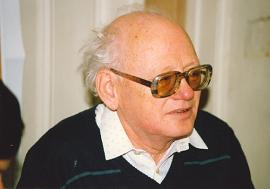
\includegraphics[height = 38mm]{figures/img/adelson-velsky.jpg}};
  \node[tannot, below = 2mm of av.south, anchor = north, align = center]
    {Georgy M. Adelson-Velsky\\[-1pt] \footnotesize (1922--2014), Moscow, 1980};

  \node[inner sep = 0pt, draw = rfaint, line width = 0.4pt,
        right = 14mm of av.east, anchor = west] (la)
    {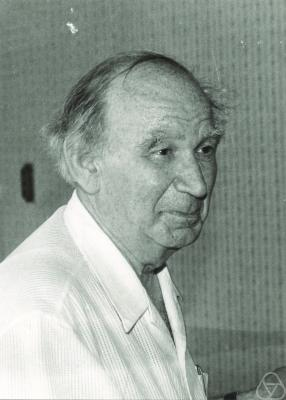
\includegraphics[height = 38mm]{figures/img/landis.jpg}};
  \node[tannot, below = 2mm of la.south, anchor = north, align = center]
    {Evgenii M. Landis\\[-1pt] \footnotesize (1921--1997)};

\end{tikzpicture}

  \caption{The authors of the 1962 paper. Left: photograph by Monroe Newborn,
  Computer History Museum Chess Collection, licensed CC BY 3.0. Right:
  photograph by Konrad Jacobs, Oberwolfach Photo Collection, licensed
  CC BY-SA 2.0 DE. Both are reproduced unaltered.}
  \label{fig:portraits}
\end{figure}

The context makes the contribution easier to see. Binary search trees were
already in use in 1962, and their weakness was understood: the shape of the tree
depends on the order the keys arrive in, and an unlucky order costs a factor of
$n$. What was missing was a way to keep the shape good without rebuilding the
tree. Adelson-Velsky and Landis supplied one, and it is the pairing of two ideas
that made it work. The first is the balance condition of \Cref{def:avl}, which is
local, so a node can be checked in constant time using information stored at that
node. The second is the rotation of \Cref{sec:rotations}, which repairs a
violation in constant time and, by \Cref{lem:inorder}, without disturbing the
search tree property. Neither idea is useful alone. Together they make the repair
affordable enough to run on every update, which is what ``self-balancing'' means.

The analysis in the original paper already contains the connection to the
Fibonacci numbers that \Cref{thm:closedform} restates, and with it the
logarithmic height bound. That the golden ratio should govern the worst-case
shape of a data structure was not an obvious thing to expect, and it remains one
of the more satisfying results in the subject: the extremal trees of
\Cref{fig:mintrees} are built by the Fibonacci recurrence because the balance
condition permits exactly a one-level gap, and a one-level gap is what turns
\Cref{eq:nrec} into \Cref{eq:mrec}.

Knuth gives the structure a detailed treatment in the second volume of
\emph{Sorting and Searching}, in the section on balanced trees~\cite{knuth3},
where the height bound appears in the form of \Cref{eq:heightbound} and the
algorithms are analysed in the level of detail that made the structure standard
teaching material.

The AVL tree has since been joined by the alternatives of
\Cref{sec:comparison}, several of which are preferred for the workloads
described in \Cref{sec:applications}. Its place is no longer automatic. What has
lasted is the method: state an invariant that can be checked locally, find a
constant-time operation that restores it, and prove that the invariant bounds the
global shape. Red-black trees, B-trees, and the rest are all built that way, and
the 1962 paper is where the pattern starts.
